\documentclass[12pt]{article}
{\usepackage{amsmath,amssymb,amsthm,enumerate,dsfont,bm}
\usepackage{pdfpages}
\usepackage[a4paper,bindingoffset=0.2in,%
left=0.8in,right=0.8in,top=1in,bottom=1in,%
footskip=.25in]{geometry}

\newcommand{\prob}[1]{\textbf{P}(#1)}
\newcommand{\ep}[1]{\mathbb{E}\left[ #1 \right]}
\newcommand{\var}[1]{var \left( #1 \right)}
\newcommand{\cp}{\overset{p}{\to}}
\newcommand{\cas}{\overset{a.s.}{\to}}
\newcommand{\cd}{\overset{D}{\to}}
\newcommand{\pard}[1]{\frac{\partial}{\partial #1}}

\title{Statistical Theory Homework 6}
\date{\today}
\author{Bohao Tang}

\begin{document}
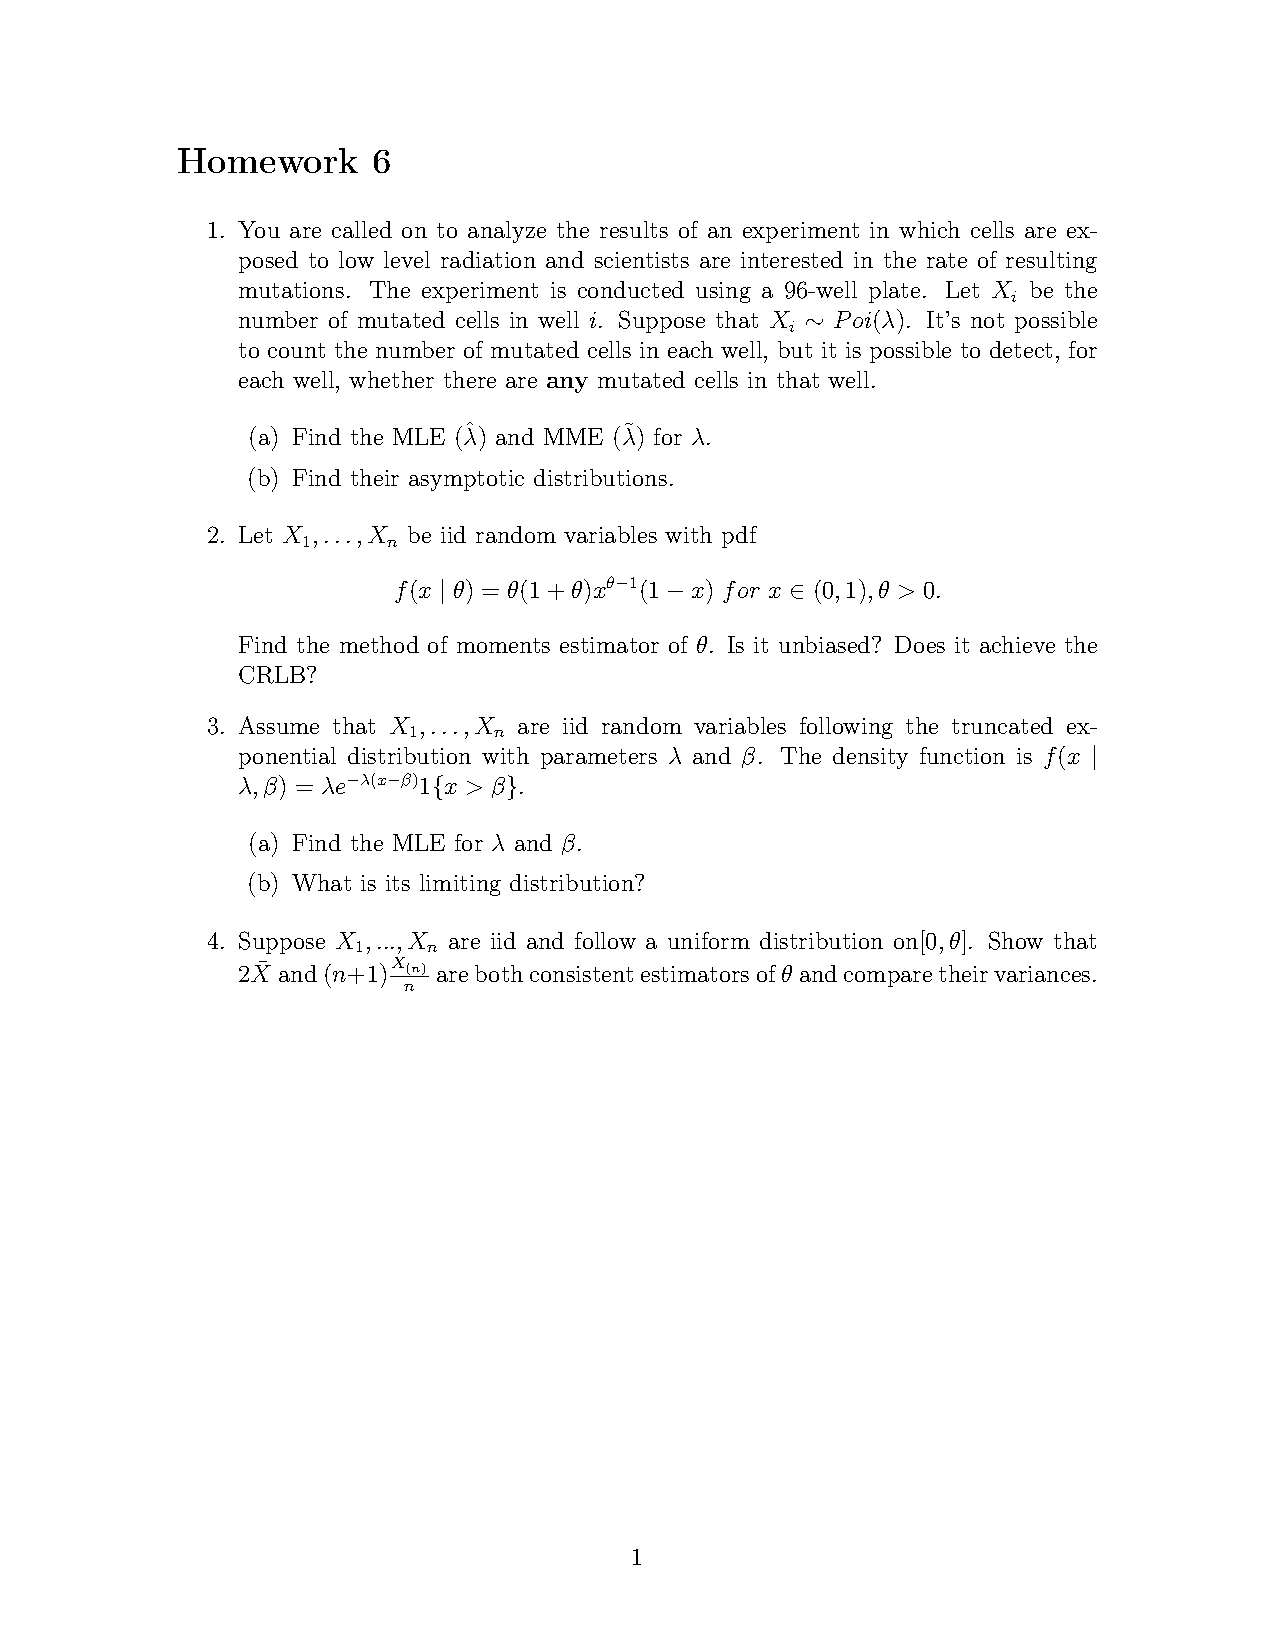
\includepdf[pages=-]{HW_6.pdf}
\maketitle

\begin{enumerate}
    \item 
    \begin{enumerate}[(a)]
        \item
        Suppose we have $n$ wells, here $n=96$. According to the setting in the question, 
        we can only observe $Y_i = \bm{1}_{X_i > 0}$. Its reasonable to suppose $X_i$ are i.i.d, 
        therefore $Y_i$ are also i.i.d random variables follow Bernoulli distribution will success probability $p = 1 - e^{-\lambda}$.

        Therefore, the likellihood of samples is $\Pi_{i=1}^n (1 - e^{-\lambda})^{Y_i} (e^{-\lambda})^{1 - Y_i}$.
        Maximize this function we get the MLE of $\lambda$ is $\hat{\lambda} = - \log(1 - \frac{\sum_1^n Y_i}{n})$.

        Also, the mean of $Y_i$ is $1 - e^{-\lambda}$, so the MME for $\lambda$ is the solution of equation $\frac{\sum_1^n Y_i}{n} = 1 - e^{-\lambda}$.
        Therefore $\tilde{\lambda} = - \log(1 - \frac{\sum_1^n Y_i}{n})$ as well.

        \item
        Since the CLT, we have $\sqrt{n} (\frac{\sum_1^n Y_i}{n} - (1 - e^{-\lambda})) \cd N(0, (1 - e^{-\lambda})e^{-\lambda})$.
        By delta method we have the asymptotic distribution of $\hat{\lambda}$ and $\tilde{\lambda}$ is:
        $$ \sqrt{n} (- \log(1 - \frac{\sum_1^n Y_i}{n}) - \lambda) \cd N(0, (e^\lambda)^2 (1 - e^{-\lambda})e^{-\lambda}) = N(0, e^\lambda - 1) $$
    \end{enumerate}

    \item
    Given $\theta$, $X$ follows beta distribution of parameter $\alpha = \theta$ and $\beta = 2$. 
    Therefore the mean of $X$ is $\frac{\alpha}{\alpha + \beta} = \frac{\theta}{\theta + 2}$. 
    The moments estimator is the solution of $\frac{\theta}{\theta + 2} = \sum_1^n X_i / n$, then we have $\hat{\theta} = \frac{\bar{X}}{1 - \bar{X}}$, where $\bar{X}$ is the sample mean.

    It is biased, for example when $n = 1$, $\hat{\theta}$ becomes $\frac{2 X_1}{1 - X_1}$. The expectation of it is $\int_0^1 \frac{2x}{1-x} \theta(\theta + 1) x^{\theta - 1}(1-x) d x = \int_0^1 2 \theta(\theta + 1) x^{\theta} d x = 2 \theta \ne \theta$. 
    So the estimator is biased.

    Also, it will not achieve the CRLB. Recall the sufficient and necessary condition for a $\theta$ estimator $w(x)$ to achieve CLRB, it is that there exists a function $a(\theta)$, such that $\pard{\theta} \log{f(x|\theta)} = a(\theta)(w(x) - \theta)$.
    We write out the likelihood:
    $$f(x|\theta) = \theta^n(1+\theta)^n \exp\{(\theta - 1) \sum \log{x_i} + \sum \log(1 - x_i)\}$$
    Then the $\pard{\theta} \log{f(x|\theta)} = \frac{n}{\theta} + \frac{n}{\theta + 1} + \sum \log{x_i}$, which can not be writen in form of $a(\theta)(\frac{2\bar{x}}{1-\bar{x}} - \theta)$. Therefore the $\hat{\theta}$ will not achieve the CRLB.

    \item
    \begin{enumerate}[(a)]
        \item
        the joint likelihood is $f(x|\lambda, \beta) = \lambda^n e^{-\lambda (\sum x_i - n \beta)} \bm{1}_{\{\forall i: \ x_i > \beta\}}$.
        Maximize this function we get the MLE estimator for $\lambda$ and $\beta$:
        \begin{eqnarray}
            \hat{\lambda} &=& \frac{1}{\bar{X} - X_{(1)}} \\
            \hat{\beta} &=& X_{(1)}
        \end{eqnarray}
        Where $\bar{X}$ is the sample mean and $X_{(1)}$ is the first order statistics.

        \item
        The distribution does not satisfy the CR regularity, so we compute the limiting distribution directly.

        First we compute the joint distribution of $\sum_1^n X_i$ and $n X_{(1)}$.
        It's known that the joint distribution of all order statistics here is $f = n! \lambda^n e^{-\lambda (\sum x_i - n\beta)} \bm{1}_{\{x_n > \cdots > x_1 > \beta\}}$

        Then we do a transformation as: 
        $$\left\{ \begin{aligned}
            y_1 &= n x_1 \\
            y_2 &= x_1 + (n-1)x_2 \\
            y_3 &= x_1 + x_2 + (n-2)x_3 \\
            &\vdots \\
            y_n &= x_1 + x_2 + x_3 + \cdots + x_n
        \end{aligned}\right.$$
        Then the density for $y_1 \cdots y_n$ is $f / |\frac{\partial (y_1 \cdots y_n)}{\partial (x_1 \cdots x_n)}| = \lambda^n e^{-\lambda (y_n - n\beta)}$, and the support is $\{y_n > y_{n-1} > \cdots > y_2 > y_1 > n\beta \}$.

        Marginalize the density on $y_1$ and $y_n$, we get that the joint distribution of $X_{(1)}$ and $\sum X_i$ is:
        $$f(y_1, y_n) = \lambda^n \frac{(y_n - y_1)^{n-2}}{(n-2)!} e^{-\lambda (y_n - n\beta)} \bm{1}_{\{y_n > y_1 > n\beta\}}$$

        Then do the transformation:
        $$\left\{ \begin{aligned}
            \hat{\lambda} &= \frac{n}{y_n - y_1} \\
            \hat{\beta} &= \frac{y_1}{n} 
        \end{aligned}\right.$$
        We get that the joint distribution of $(\hat{\lambda}, \hat{\beta})$ is:
        $$f(z_1, z_2) = \frac{\lambda^n n^n}{(n-2)! z_1^n} e^{-\lambda n / z_1}  \bm{1}_{z_1 > 0} \times e^{-n\lambda(z_2 - \beta)} \bm{1}_{z_2 > \beta}$$
        Since $f(z_1, z_2)$ can be factorized into production of function of $z_1$ and function of $z_2$, we know that $\hat{\lambda}$ and $\hat{\beta}$ are independent. 

        By the factorization, we know that $n (\hat{\beta} - \beta) \sim \exp(\lambda)$, therefore $\sqrt{n} (\hat{\beta} - \beta) \cd 0$.
        Recall the CLT we have that $\sqrt{n}\left\{\bar{X} - (\frac{1}{\lambda} + \beta)\right\} \cd N(0, \frac{1}{\lambda^2})$, by Slutsky's Theorem we have:
        $$\sqrt{n}(\bar{X} - X_{(1)} - \frac{1}{\lambda}) = \sqrt{n}(\bar{X} - \frac{1}{\lambda} - \beta) - \sqrt{n}(X_{(1)} - \beta) \cd N(0, \frac{1}{\lambda^2})$$
        By delta method we have:
        $$\sqrt{n}(\hat{\lambda} - \lambda) \cd N(0, \lambda^2)$$

        In conclusion, the estimators $\hat{\lambda}$ and $\hat{\beta}$ are consistent and mutual independent. But they are not in the same scale.
        \begin{eqnarray}
            n (\hat{\beta} - \beta) &\cd& \exp(\lambda) \\
            \sqrt{n}(\hat{\lambda} - \lambda) &\cd& N(0, \lambda^2)
        \end{eqnarray}

    \end{enumerate}

    \item
    By the WLLN we have that $\bar{X} \cp \ep{X} = \theta /2$, so $2 \bar{X} \cp \theta$, which means $2\bar{X}$ is consistent.

    For every $\gamma < \theta$, we have that $\prob{\gamma < X_{(n)} \le \theta} = 1 - (\frac{\gamma}{\theta})^n \to 1$, therefore $X_{(n)} \cp \theta$.
    By Slutsky's Theorem, we have $(n+1)\frac{X_{(n)}}{n} \cp \theta$, so it's also consistent.

    Now we compute their variance:
    $$\var{2 \bar{X}} = \frac{4}{n} \var{X_1} = \frac{\theta^2}{3 n}$$
    And:
    \begin{eqnarray}
        \var{\frac{n+1}{n} X_{(n)}} &=& (\frac{n+1}{n})^2 \left\{(\int_0^\theta t^2 \frac{n t^{n-1}}{\theta^n} d t) - (\int_0^\theta t \frac{n t^{n-1}}{\theta^n} d t)^2 \right\} \\        
                                    &=& (\frac{n+1}{n})^2 \left(\frac{n}{n+2} \theta^2 - (\frac{n}{n+1} \theta)^2 \right) \\
                                    &=& \frac{\theta^2}{n(n+2)}
    \end{eqnarray}
    We get that $\var{\frac{n+1}{n} X_{(n)}} < \var{2 \bar{X}}$ when $n > 1$, so estimator $\var{\frac{n+1}{n} X_{(n)}}$ is more efficient.

\end{enumerate}
    
\end{document}